% Options for packages loaded elsewhere
\PassOptionsToPackage{unicode}{hyperref}
\PassOptionsToPackage{hyphens}{url}
\PassOptionsToPackage{dvipsnames,svgnames*,x11names*}{xcolor}
%
\documentclass[
  spanish,
  a4paper,
  openany]{book}
\usepackage{amsmath,amssymb}
\usepackage[]{bookman}
\usepackage{ifxetex,ifluatex}
\ifnum 0\ifxetex 1\fi\ifluatex 1\fi=0 % if pdftex
  \usepackage[T1]{fontenc}
  \usepackage[utf8]{inputenc}
  \usepackage{textcomp} % provide euro and other symbols
\else % if luatex or xetex
  \usepackage{unicode-math}
  \defaultfontfeatures{Scale=MatchLowercase}
  \defaultfontfeatures[\rmfamily]{Ligatures=TeX,Scale=1}
\fi
% Use upquote if available, for straight quotes in verbatim environments
\IfFileExists{upquote.sty}{\usepackage{upquote}}{}
\IfFileExists{microtype.sty}{% use microtype if available
  \usepackage[]{microtype}
  \UseMicrotypeSet[protrusion]{basicmath} % disable protrusion for tt fonts
}{}
\makeatletter
\@ifundefined{KOMAClassName}{% if non-KOMA class
  \IfFileExists{parskip.sty}{%
    \usepackage{parskip}
  }{% else
    \setlength{\parindent}{0pt}
    \setlength{\parskip}{6pt plus 2pt minus 1pt}}
}{% if KOMA class
  \KOMAoptions{parskip=half}}
\makeatother
\usepackage{xcolor}
\IfFileExists{xurl.sty}{\usepackage{xurl}}{} % add URL line breaks if available
\IfFileExists{bookmark.sty}{\usepackage{bookmark}}{\usepackage{hyperref}}
\hypersetup{
  pdftitle={Manual de privacidad y seguridad en internet},
  pdfauthor={Diego Chiquero Mena},
  pdflang={es},
  pdfkeywords={seguridad,privacidad, ciberdelitos, ciberdelincuentes,internet},
  colorlinks=true,
  linkcolor=blue,
  filecolor=Maroon,
  citecolor=Blue,
  urlcolor=Blue,
  pdfcreator={LaTeX via pandoc}}
\urlstyle{same} % disable monospaced font for URLs
\usepackage[top=1in,bottom=1in,right=1in,left=1in]{geometry}
\usepackage{longtable,booktabs,array}
\usepackage{calc} % for calculating minipage widths
% Correct order of tables after \paragraph or \subparagraph
\usepackage{etoolbox}
\makeatletter
\patchcmd\longtable{\par}{\if@noskipsec\mbox{}\fi\par}{}{}
\makeatother
% Allow footnotes in longtable head/foot
\IfFileExists{footnotehyper.sty}{\usepackage{footnotehyper}}{\usepackage{footnote}}
\makesavenoteenv{longtable}
\usepackage{graphicx}
\makeatletter
\def\maxwidth{\ifdim\Gin@nat@width>\linewidth\linewidth\else\Gin@nat@width\fi}
\def\maxheight{\ifdim\Gin@nat@height>\textheight\textheight\else\Gin@nat@height\fi}
\makeatother
% Scale images if necessary, so that they will not overflow the page
% margins by default, and it is still possible to overwrite the defaults
% using explicit options in \includegraphics[width, height, ...]{}
\setkeys{Gin}{width=\maxwidth,height=\maxheight,keepaspectratio}
% Set default figure placement to htbp
\makeatletter
\def\fps@figure{htbp}
\makeatother
\setlength{\emergencystretch}{3em} % prevent overfull lines
\providecommand{\tightlist}{%
  \setlength{\itemsep}{0pt}\setlength{\parskip}{0pt}}
\setcounter{secnumdepth}{5}
\usepackage{graphicx}
\usepackage{fancyhdr}
\pagestyle{plain}
\renewcommand{\headrulewidth}{0.2pt}
\usepackage{floatpag}
\floatpagestyle{empty}
\ifxetex
  % Load polyglossia as late as possible: uses bidi with RTL langages (e.g. Hebrew, Arabic)
  \usepackage{polyglossia}
  \setmainlanguage[]{spanish}
\else
  \usepackage[main=spanish]{babel}
% get rid of language-specific shorthands (see #6817):
\let\LanguageShortHands\languageshorthands
\def\languageshorthands#1{}
\fi
\ifluatex
  \usepackage{selnolig}  % disable illegal ligatures
\fi
\usepackage[]{natbib}
\bibliographystyle{apalike}

\title{Manual de privacidad y seguridad en internet}
\author{Diego Chiquero Mena}
\date{26 enero 2021}

\begin{document}
\maketitle

\thispagestyle{empty}
\begin{center}
\noindent\makebox[\textwidth]{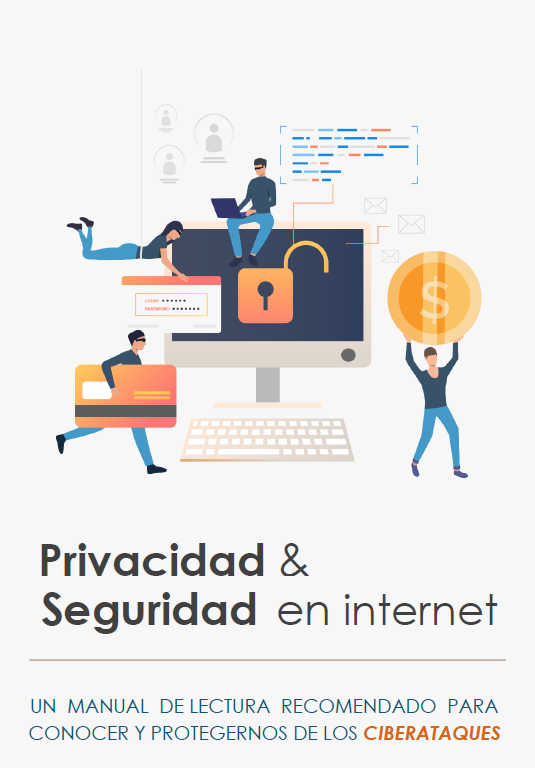
\includegraphics[width=\paperwidth]{images/cover.png}}
%\makebox[\textwidth]{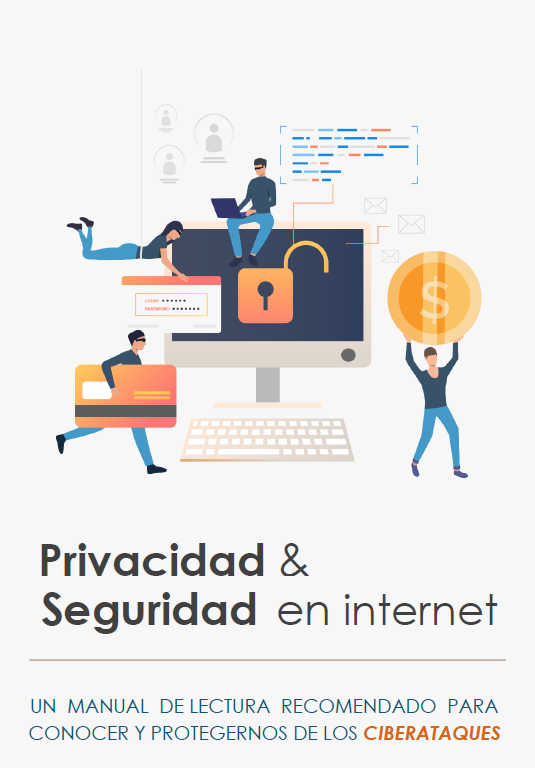
\includegraphics[width=\paperwidth]{images/cover.png}}
\end{center}
\fontsize{14}{16}
%\fontseries{b}
\selectfont





{
\hypersetup{linkcolor=}
\setcounter{tocdepth}{3}
\tableofcontents
}
\hypertarget{pruxf3logo}{%
\chapter*{Prólogo}\label{pruxf3logo}}
\addcontentsline{toc}{chapter}{Prólogo}

Este manual aglutina de manera filtrada y tamizada una amplia y detallada parte del conocimiento e información de relevancia que puedes encontrar en la web sobre privacidad y seguridad en internet, de forma ordenada y estructura. Además encontrarás en la bibliografía todas las fuentes que han hecho posible la elaboración y documentación de este manual, para que puedas contrastar por ti mismo dichas fuentes.

Entenderás las diferencias entre los conceptos de privacidad y seguridad en internet, para que de este modo puedas hacer una buena configuración y uso de éstas.

Aprenderás buenas prácticas en la gestión de la privacidad, así como la manera más adecuada de gestionar la seguridad tanto en los equipos (PC, tables, smartphones, etc.), como en la red de datos.

Conocerás las principales amenazas que existen en el uso de las tecnologías y el mundo digital.

Y por último, pero no por ello menos importante, se abordarán otros conceptos relacionados con los ciberdelitos, la huella digital, la importancia de ser selectivos con la información online y otros aspectos más.

Para concluir, también encontrarás a lo largo del manual multitud de enlaces que te llevarán a más información ampliada sobre las temáticas, así como una extensa lista de recursos y herramientas para que puedas llevar tu privacidad y seguridad en internet al siguiente nivel.

Si quieres contribuir y ayudar a nutrir de más contenido de valor este manual, por favor, no lo dudes y ponte en contacto conmigo, estaré encantado que colaboremos. Encontrarás mis datos de contacto en el siguiente apartado \emph{sobre el autor}.

Este manual está disponible en el repositorio Github: \href{https://github.com/diegochiquero/manual-de-privacidad-y-seguridad-en-internet}{diegochiquero/manual-de-privacidad-y-seguridad-en-internet}. Y ha sido escrito en \href{http://rmarkdown.rstudio.com}{R-Markdown} empleando el paquete \href{https://bookdown.org/}{\texttt{bookdown}} cuya guia encontrarás en \citep{R-bookdown}.

Imagen portada \citep{freepik}

Esta obra está bajo la \href{https://creativecommons.org/licenses/by-nc-sa/4.0/deed.es}{licencia Creative Commons Atribución-NoComercial-CompartirIgual 4.0 Internacional}.

\begin{flushleft}
\includegraphics{images/by-nc-sa-88x31} \end{flushleft}

\hypertarget{autor}{%
\chapter*{Sobre el autor}\label{autor}}
\addcontentsline{toc}{chapter}{Sobre el autor}

\begin{flushleft}
\includegraphics[width=0.25\linewidth]{images/diego-chiquero-2020-profile} \end{flushleft}

Hola, mi nombre en Diego.

Y lo primero que me gustaría hacer, es agradecerte que hayas decidido leer este manual. Ya que éste hecho, hace que las horas de dedicación, esfuerzo, documentación y contrastación de fuentes hayan merecido la pena.

El propósito de este manual es hacerte consciente de los peligros de navegar por internet, de lo vulnerable y expuesto que puedes llegar a estar en el uso de las tecnologías y a su vez dotarte de conocimientos, consejos y herramientas para poder hacer una buena gestión de la web de manera segura y privada.

De formación académica Técnico superior en desarrollo de aplicaciones web.
Para concluir y a modo de breve presentación, haré referencia a mi extracto de Linkedin:

\begin{quote}
Apasionado de las tecnologías, el espíritu empresarial y la programación.

Plenamente convencido que las competencias transversales pueden marcan la diferencia, que el derecho nos asiste a todos y que un mundo mejor es posible.

En continuo proceso de crecimiento personal y profesional.
\end{quote}

Diego Chiquero Mena

Puedes contactar conmigo en \href{mailto:chiquerodiego@yahoo.es}{\nolinkurl{chiquerodiego@yahoo.es}}

Más sobre mí \href{https://about.me/diegochiquero}{Diego Chiquero Mena}

\hypertarget{privacidad-y-seguridad-en-internet}{%
\chapter{Privacidad y Seguridad en Internet}\label{privacidad-y-seguridad-en-internet}}

\hypertarget{introducciuxf3n}{%
\section{Introducción}\label{introducciuxf3n}}

En estos últimos años hemos podido ver como la evolución de las IT (Tecnologías de la información) y el paso de la Web1.0. a la Web 2.0., nos ha permitido a muchos de nosotros como usuarios interactuar los unos con los otros subiendo y compartiendo todo tipo de contenidos. La aparición de las Redes sociales ha traído con ellas, la posibilidad de publicar fotos, videos, información, comentarios, reseñas, etc. a través de cualquier dispositivo, ya sea un PC, tablet o smartphone. Y no solo eso, sino que además, también nos ha abrierto un amplio abanico de posibilidades con las que podemos gestionar cuentas bancarias, hacer compras online, trámites telemáticos y un sinfín de gestiones que hasta hace tan solo unos años atrás eran difíciles de imaginar.

Como consecuencia de ello, el enorme conglomerado de información sensible que se encuentra disponible en internet, hace que nosotros como usuarios estemos en el punto de mira de ciberdelincuentes y expuestos a todo tipo de ciberataques. En esta línea, este manual contribuye a enseñarte, aconsejarte y proveerte de herramientas necesarias para prevenir, evitar y paliar en la medida de lo posible todos los riesgos y peligros a los que estamos expuestos en nuestro uso diario de las tecnologías.

Por lo tanto, en lo sucesivo iras viendo el porqué de la importancia de velar de manera activa por tu privacidad y seguridad en internet haciendo una buena gestión de éstas. También te ayudará a conocer y reconocer la amplia lista de ciberdelitos que actualmente están más extendidos.

En estás \href{https://oedi.es/estadisticas/}{estadísticas} públicadas por el Obsevatorio Español de Delitos informáticos \citep{oedi} puedes ver el porqué de cuidar tu privacidad y seguridad en internet. En ellas se expone una exhaustiva lista de ciberdelitos y sus recurrencias cronológicas.

\hypertarget{privacidad}{%
\section{Privacidad}\label{privacidad}}

La privacidad es aquello que se lleva a cabo en un ámbito reservado; en Internet podría entenderse como el control que ejercemos sobre nuestra información para limitar la cantidad de personas autorizadas a verla, así como la cantidad de contenido expuesto. Esto incluye datos personales, fotografías, documentos, etc.

Internet es una herramienta que nos permite la interacción entre dos o más personas. Siendo ejemplo de los anteriores sitios como Facebook y Twitter, Redes Sociales en donde las personas pueden compartir públicamente opiniones, noticias, sentimientos, ideas, fotografías, videos, etc. Por ello es necesario considerar que Internet es un espacio abierto al mundo, por lo tanto, cualquier acción que se haga va a tener un impacto global y permanente. Por ejemplo, imagina una publicación de la cual puedas arrepentirte (como una fotografía u opinión) no solo podrá ser vista por millones de usuarios , sino que también será prácticamente imposible de borrar completamente de la red .

También puede resultar peligroso publicar datos que puedan identificarte, como la dirección, teléfonos, lugar de estudio o trabajo, días de vacaciones, etc. Esto puede resultar todavía más complicado si posees una gran lista de amigos a los que no conoces personalmente.

Por todo lo que se ha mencionado en éstas últimas líneas, es de suma importancia que antes de publicar algo, pienses en las consecuencias que puede conllevar divulgar información sensible en sitios públicos y de los cuales no siempre se tiene un control directo \citep{privacidad}.

\hypertarget{seguridad}{%
\section{Seguridad}\label{seguridad}}

La seguridad en internet son todas aquellas precauciones que son tomadas para proteger todos los dispositivos informáticos, así como la red de internet que pueden ser afectados por delincuentes cibernéticos. Además de ser una rama de la seguridad informática que se dedica a identificar y prevenir todas las amenazas que afectan a la red de redes, siendo una de las herramientas más conocidas los antivirus \citep{seguridad}.

Entre los peligros más habituales de no hacer un buen uso de la seguridad en la red, nos encontramos, robo de datos bancarios o personales, virus informáticos, phishing, spam, etc. Una lista amplia y exhaustiva será vista la unidad \ref{amenazas} Amenazas.

\hypertarget{rgpd-reglamento-general-de-protecciuxf3n-de-datos}{%
\section{RGPD (Reglamento general de protección de datos)}\label{rgpd-reglamento-general-de-protecciuxf3n-de-datos}}

El Reglamento General de Protección de Datos (RGPD) es el reglamento europeo relativo a la protección de las personas físicas en lo que respecta al tratamiento de sus datos personales y a la libre circulación de estos datos. Entró en vigor el 25 de mayo de 2016 y fue de aplicación el 25 de mayo de 2018, dos años durante los cuales las empresas, las organizaciones, los organismos y las instituciones han debido ir adaptándose para su cumplimiento. Es una normativa a nivel de la Unión Europea, por lo que cualquier empresa de la unión, o aquellas empresas que tengan negocios en la Unión Europea, que manejen información personal de cualquier tipo deberán acogerse a la misma \citep{rgpd}.

En el pasado el uso de datos eran obtenido por omisión, en estos momentos para estar seguros de cumplir con el RGPD se ha de obtener el consentimiento inequívoco o expreso por parte del usuario.

Paralela a la RGPD europea existe una a nivel de España llamada LOPD (Ley orgánica de protección de datos).

\hypertarget{aviso-legal-poluxedtica-de-privacidad-y-poluxedtica-de-cookies}{%
\section{Aviso legal, política de privacidad y política de cookies}\label{aviso-legal-poluxedtica-de-privacidad-y-poluxedtica-de-cookies}}

Si una web va a realizar transacciones comerciales de la naturaleza que sea, va a gestionar datos de usuarios o hacer uso de cookies, ha de tener a disposición del usuario la siguiente información de manera detallada. Todas estas políticas están recogidas en el RGPD del apartado anterior. Sin embargo para documentarlo con terminología más cotidiana, en este apartado nos hemos apoyado en la sección de derecho digital de la compañía IONOS by 1\&1 en su división IONOS Guía Digital,

\begin{itemize}
\item
  Aviso Legal: Se trata de un documento donde se recogen tanto el cumplimiento por parte de la entidad o empresa, conforme a las leyes vigentes en el desarrollo de su actividad, así como los datos referentes a los administradores de la misma.

  Todo proyecto de base digital u online con ánimo de lucro, ya sea a través de modelos de patrocinio, publicitarios o compra-venta de productos o servicios, requieren de un aviso legal visiblemente expuesto y a disposición de todos los usuarios. Este requerimiento está recogido en la legislación española en la Ley 34/2002 de Servicios de la Sociedad de la Información y el Comercio Electrónico \citep{legal}.
\item
  Política de privacidad: El reglamento general de Protección de Datos de carácter personal, establece que cualquier página web que incluya un formulario de carácter personal que deban rellenar los usuarios, que incluya un correo de contacto o utilice las redes sociales desde las cuales se puede obtener información de los usuarios, está obligada a disponer de una política de privacidad \citep{p-privacidad}.

  La política de privacidad se creó con la finalidad de proteger y preservar los derechos del espacio privado de las personas.
\item
  Política de cookies: Una cookie es una pequeña información enviada por un sitio web y almacenado en el navegador del usuario, de manera que el sitio web puede consultar la actividad previa del navegador. Su propósito principal es identificar al usuario almacenando su historial de actividad en un sitio web específico, de manera que se le pueda ofrecer el contenido más apropiado según sus hábitos \citep{cookies}.

  Toda web que haga uso de cookies está obligada ponerlo en conocimiento de los usuarios y a solicitar su aceptación.
\end{itemize}

\hypertarget{gestiuxf3n-de-la-privacidad}{%
\chapter{Gestión de la privacidad}\label{gestiuxf3n-de-la-privacidad}}

\hypertarget{gestionando-la-privacidad}{%
\section{Gestionando la privacidad}\label{gestionando-la-privacidad}}

Este es otro ejemplo de índice\footnote{Esta es la explicación sin más}.

\hypertarget{datos-personales-sensibles}{%
\section{Datos personales sensibles}\label{datos-personales-sensibles}}

Hiperlink de ejemplo \href{https://www.google.com}{Google}

\hypertarget{oversharing}{%
\section{Oversharing}\label{oversharing}}

Esto es un texto normal que contiene una nota\footnote{Aquí irá el texto de tu nota.}. Puedes escribir tanto como necesites.

\hypertarget{privacidad-en-tus-cuentas}{%
\section{Privacidad en tus cuentas}\label{privacidad-en-tus-cuentas}}

Cuentas

\hypertarget{navegaciuxf3n-privada}{%
\section{Navegación privada}\label{navegaciuxf3n-privada}}

La navegación

\hypertarget{cookies}{%
\section{Cookies}\label{cookies}}

La cookies son \ldots{}

\hypertarget{la-nube}{%
\section{La nube}\label{la-nube}}

Que pasa en la nube

Incluso crear varios párrafos, ya que la nota siempre irá al final del documento. En este caso, si haces click serás dirigido al final del artículo (pero puedes volver al punto de lectura fácilmente, ¡haz la prueba!)

\hypertarget{gestiuxf3n-de-la-seguridad-en-equipos-fuxedsicos}{%
\chapter{Gestión de la seguridad en equipos físicos}\label{gestiuxf3n-de-la-seguridad-en-equipos-fuxedsicos}}

\hypertarget{gestionando-la-seguridad-en-los-equipos}{%
\section{Gestionando la seguridad en los equipos}\label{gestionando-la-seguridad-en-los-equipos}}

Para poder tener la tranquilidad de que tus equipos tales, como el ordenador, la tablet, el smartphone, el router, etc., estén a salvo de ataques o pérdidas de datos, entre otras, debes mantener una seguridad robusta y confiable en tus equipos.

A lo largo de esta unidad veras que debes hacer y las precauciones que debes tomar para que tus equipos e información estén seguros y a salvo de ciberataques.

\hypertarget{equipo-local-y-dispositivos-muxf3viles}{%
\section{Equipo local y dispositivos móviles}\label{equipo-local-y-dispositivos-muxf3viles}}

Una cuenta de usuario es el conjunto de información perteneciente a un usuario concreto. De esta forma indica al sistema operativo los archivos y carpetas a los que dicho usuario tiene acceso así como la posibilidad de realizar cambios y configuraciones personales \citep{OSI-cuentas}.

Las pautas de seguridad que vas a ver a continuación te van a ser útil, tanto para ordenadores como cualquier tipo de dispositivo móvil, smartwatch y demás.

Todos los equipos informáticos funcionan con una cuenta de usuario, única y personal. Luego una vez, hayas creado la tuya, solo tú debes hacer uso y disfrute de ella. En los ordenadores personales existe la posibilidad de crear varias cuentas de usuarios. Una vez éstas están creadas solo son accesibles mediante contraseña y aunque solo sirva para no olvidarlo, nunca debes de compartida.

\begin{figure}

{\centering 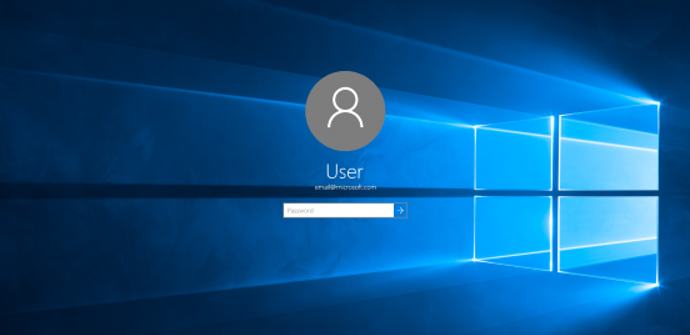
\includegraphics[width=1\linewidth]{images/cuenta-usuario-windows-10} 

}

\caption{Cuenta de usuario windows 10.}\label{fig:rmarkdown}
\end{figure}

\hypertarget{router}{%
\section{Router}\label{router}}

Un router es un dispositivo que proporciona conectividad a nivel de red. Su función principal consiste en enviar o encaminar paquetes de datos de una red a otra, es decir, interconectar subredes, entendiendo por subred un conjunto de máquinas IP que se pueden comunicar. Además de ser el dispositivo que nos proporciona un punto de acceso Wi-Fi

Dispone de varios niveles de seguridad y estándares de cifrado, para que nadie pueda acceder a nuestra red y poder alcanzar cualquier dispositivo a través d la Wi-Fi.

Ordenados de menor a mayor grado de cifrado:

\begin{itemize}
\tightlist
\item
  WEP (Wired Equivalent Privacy)
\item
  WPA (Wi-Fi Protected Access)
\item
  WPA2 (Wi-Fi Protected Access 2)
\end{itemize}

Es importante que cambies la clave que el router trae por defecto y uses el nivel de seguridad WPA2 con el que vas a poder establecer una contraseña de hasta 63 caracteres en lugar de los máximos 29 de la WEP.1

Para establecer una capa más de seguridad puedes realizar un filtrado MAC (Media Access Control). Un filtra MAC consiste en la creación de una lista de dispositivos que tienen permiso para acceder al router, a pesar de que un tercero haya podido obtener la clave wifi.

\hypertarget{actualizaciones}{%
\section{Actualizaciones}\label{actualizaciones}}

Las actualizaciones de seguridad o parches son elaboradas por los desarrolladores y fabricantes de productos informáticos. Estos pueden tardar desde un día hasta meses para publicar un parche, en función del tipo de vulnerabilidad, dispositivos a los que afecte y otros criterios. Aunque también se realizan para mejoras de otras naturalezas, como, rendimiento, productividad, etc.

Tener actualizados los dispositivos es una medida más de seguridad. Para ello debes actualizarlos cada vez que el dispositivo lo solicita o en su defecto buscar una actualización disponible.

Las actualizaciones no solo corresponden al Hardware (ordenadores, smartphones, etc.), sino que también han de ser realizados en el software (programas), navegadores, antivirus, etc.

\hypertarget{antivirus-antimalware-antispyware-y-firewall}{%
\section{Antivirus, antimalware, antispyware y firewall}\label{antivirus-antimalware-antispyware-y-firewall}}

Aunque a priori pudiese parecer lo mismo, los antivirus, antimalware, antispyware y firewall, cumple funciones diferentes, pero con un mismo fin, mantener la seguridad de nuestros equipos. La mayoría de estos tipos de software los puedes encontrar en dos modalidades: gratuita y de pago.1

\begin{itemize}
\item
  Antivirus: Es un programa que detecta la presencia de virus informáticos (software malicioso que altera el funcionamiento normal del ordenador sin que el usuario lo sepa o consienta) y los elimina o repara. Algunos ejemplos de antivirus son: Avira, Avast, AVG, Virus Total (online), entre muchos más.
\item
  Firewall o cortafuegos: Es una parte de la red o el sistema que se realiza para bloquear accesos no autorizados y permitiendo los que sí lo están. Se pueden hacer por medio de software o hardware, y permiten una mayor protección a las redes, especialmente importante en empresas que cuentan con datos que han de ser bien protegidos. El firewall más conocido es el Windows.
\item
  Antispyware: Es un conjunto de herramientas que sirven para prevenir y eliminar Spywares (espías o programas que recopilan información del ordenador para transmitirla a otras personas sin el consentimiento ni conocimiento del propietario del ordenador). Algunos ejemplos de antispyware son: SpyBot, SuperAntiSpyware, SpywareBlaster.
\item
  Antimalware: Es un software encargado de eliminar el software malicioso (malicious-software, malware) del ordenador tras un minucioso análisis del sistema. Algunos ejemplos de antimalware son: HiJackThis, Anti-malware.
\end{itemize}

Dependiendo de las necesidades pueden ser usados uno o varios, ya que son complementarios entre sí.

\hypertarget{copias-de-seguridad}{%
\section{Copias de seguridad}\label{copias-de-seguridad}}

Una copia de seguridad o backup en informática es una copia de los datos originales que se realiza con el fin de disponer de un medio para recuperarlos en caso de su pérdida. Las copias de seguridad son útiles ante distintos eventos y usos: recuperar los sistemas informáticos y los datos de una catástrofe informática, natural o ataque; restaurar una pequeña cantidad de archivos que pueden haberse eliminado accidentalmente, corrompido, infectado por un virus informático u otras causas.1

Simplificando el sistema de copias de seguridad que en algunas ocasiones puede llegar a ser complejo, están los siguiente:

\begin{itemize}
\item
  Completas: Del sistema operativo completo, de esta forma al restaurar la copia, dispondremos de nuevo de toda la configuración a nivel de S.O., software instalado, carpetas y archivos. Para este cometido vamos a necesitar de programas de terceros, algunos de ellos con versiones gratuitas y de pago, ejemplo de estos son: Acronis, AOMEI, EaseUS.
\item
  Parciales: En este escenario lo que se hace es salvaguardar las carpetas y archivos personales. Como por ejemplo, carpetas con fotografías, documentos personales y demás.
\end{itemize}

Y las copias pueden ser mantenidas:

\begin{itemize}
\item
  En almacenamientos externos: Tales como disco duros externos, DVD, entre otros. De esta forma podemos custodiarlos a buen recaudo.
\item
  En la nube: Estos son servicios de terceros accesibles online, ejemplo de ello son: BackBlaze, Carbonite, siendo estos especializados en backups. Pero si tus copias de seguridad se limitan a tus carpetas y archivos personales puedes usar un servicio en la nube, como Google Drive, Onedrive o Dropbox.
\end{itemize}

Las copias de seguridad debes realizarlas con la frecuencia que sea necesaria para garantizar tu nivel de seguridad.

\hypertarget{applicaciones}{%
\chapter{Applicaciones}\label{applicaciones}}

Some \emph{significant} applications are demonstrated in this chapter.

\hypertarget{segundo-nivel}{%
\section{Segundo nivel}\label{segundo-nivel}}

Segundo nivel

\hypertarget{tercer-nivel}{%
\subsection{Tercer nivel}\label{tercer-nivel}}

Tercer nivel

\hypertarget{cuarto-nivel}{%
\subsubsection{Cuarto nivel}\label{cuarto-nivel}}

Cuarto nivel

\hypertarget{segundo-nivel-b}{%
\section{Segundo nivel B}\label{segundo-nivel-b}}

\hypertarget{amenazas}{%
\chapter{Amenazas}\label{amenazas}}

We have finished a nice book.

You can write citations, too. For example, we are using the \textbf{bookdown} package in this sample book, which was built on top of R Markdown and \textbf{knitr}.

\hypertarget{otro}{%
\chapter{Otro}\label{otro}}

Esta es la última unidad

For example, we are using the \textbf{bookdown} package \citep{R-bookdown} in this sample book

Ejemplos de este tipo de libros\footnote{Los libros de Hadley \href{http://adv-r.had.co.nz}{Advanced R} y \href{http://r-pkgs.had.co.nz}{R packages}
  serían ejemplos con una versión ``preliminar'' de este paquete.} se tienen en \url{https://bookdown.org} (el listado completo está disponible \href{https://bookdown.org/home/archive/}{aquí}).

Y en Linux\footnote{Aunque el autor del paquete \texttt{bookdown} recomienda instalar \href{https://yihui.name/tinytex}{TinyTeX}.}.

\begin{verbatim}
You can add text to your text as follows.
\end{verbatim}

  \bibliography{book.bib,article.bib,manual.bib}

\end{document}
